
\documentclass{acm_proc_article-sp}
%documentclass{article}
\begin{document}

\title{Paragraph: A Paravirtual Graphics Card in Palacios}
\numberofauthors{3} %  in this sample file, there are a *total*
\author{
% 1st. author
\alignauthor
Ruba Merza\\
       \affaddr{Northwestern University}\\
       \affaddr{1117 Forest Avenue}\\
       \affaddr{Evanston, IL, 60202}\\
       \email{ruba@u.northwestern.edu}
% 2nd. author
\alignauthor
Ross Freiman\\
       \affaddr{Northwestern University}\\
       \affaddr{2234 Sherman Ave.}\\
       \affaddr{Evanston, IL, 60201}\\
       \email{rossfreiman2013@u.northwestern.edu}
% 3rd. author
\alignauthor
Ketaki Joshi\\
       \affaddr{Northwestern University}\\
       \affaddr{1 Th{\o}rv{\"a}ld Circle}\\
       \affaddr{Hekla, Iceland}\\
       \email{larst@affiliation.org}
}

\maketitle
\begin{abstract}
The focus of this paper is implementing a paravirtual graphics card and an X11 device driver for
a virtual machine monitor called Palacios. While Palacios implements a VGA graphics card with
a complex interface to the virtual guest, a paravirtual graphics card provides a simple interface
by writing directly an array of pixels into a chunk of memory, called the framebuffer, which is then
read by an X11 server and rendered onto the screen through an X11 client.
This paper looks at the current implementation of graphics in Palacios and describes the new
implementation with a paravirtual graphics card. It also provides a short description of the X
client\--­server model and the X11 driver written for the paravirtual graphics card.
\end{abstract}

\category{H.4}{Virtualization}{Systems}
\terms{Documentation, Design, Experimentation, Theory}
\keywords{Paravirtual, Graphics, Graphics Card, X11, Palacios, Virtual Device}

\section{Introduction}
The goal of this paper is to describe an implementation of a paravirtual
graphics card for Palacios, an OS independent open source virtual machine
monitor. \cite{Lange: Technical} Palacios is designed to be 
highly configurable and provides a suitable environment
for prototyping new extensions and devices. Palacios currently implements
  a virtual VGA card whose interface to the guest VM is very elaborate. The
  purpose of a paravirtual graphics card is to eliminate such complex interface
  by providing a much simpler and more compact one to the guest that can
  consequently make for a substitute for the VGA card altogether. In addition to
  replacing the VGA in Palacios, the paravirtual graphics card's manageable
  interface makes it easy to configure it with an X11 device driver and thus
  enables us to harness the capabilities of the X11 window system and run it with the
  graphics card within a virtual guest. In the following sections we go into
  detail about Palacios' current implementation of graphics, the paravirtual
  graphics card's interface, the X11 window system, and the steps we took in
  building such graphics card and running X on a virtual guest.

\section{Graphics in Palacios}
The way graphics currently work on Palacios comprises of three main components.
The VGA device, the graphics console, and the VNC server/client. In the
following subsection we will give an overview of the VGA device, followed by two
subsections, one describing the graphics console and the other describing the
VNC server/client used in Palacios.
 TODO: explain the figure
\begin{figure}[h]                                              
\centering                                                 
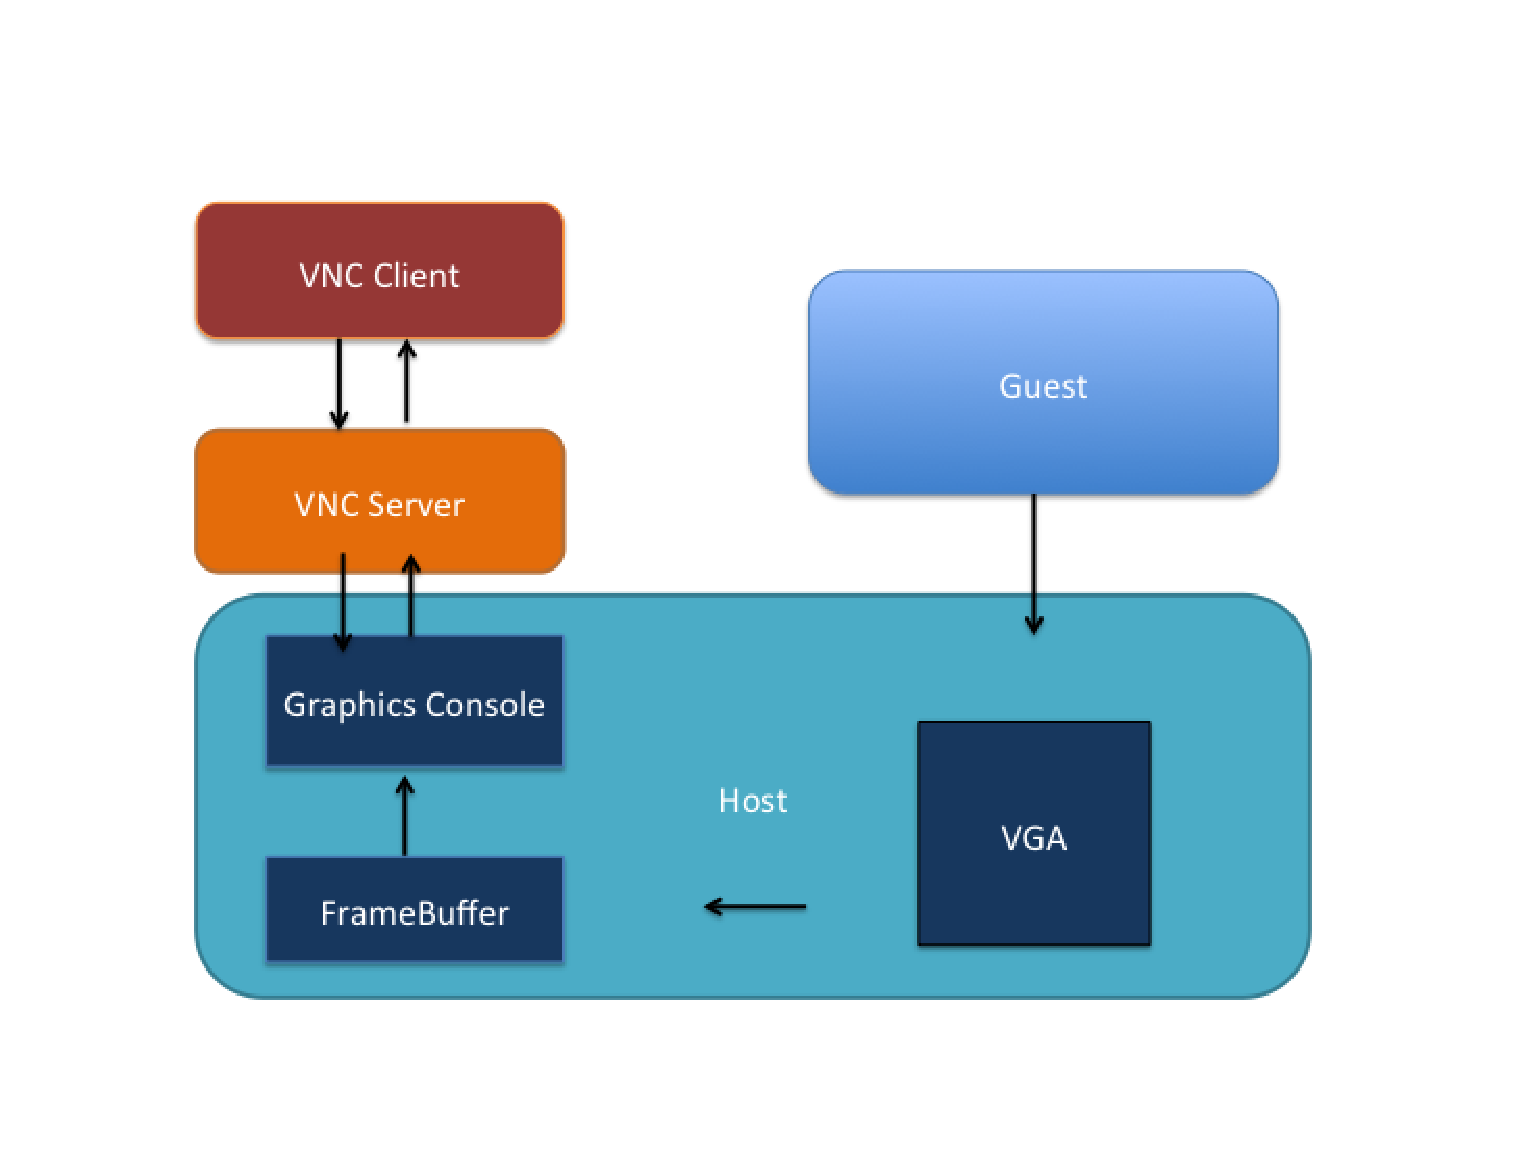
\epsfig{file=VGA.eps, height=3in, width=4in}                                      
\caption{A model of how graphics work currently in Palacios}   
\end{figure}                                               

\subsection{VGA}

\subsection{The Graphics Console} % can add more about its functions
The Graphics Console interface interfaces with a VM's text\--mode and graphics
mode display adaptor (e.g. VGA), keyboard, and mouse to allow the host OS to display the VM
console as appropriate. In the Linux module, the graphics console interface implementation provides
for a userspace utility to attach to a frame buffer. The utility then exports this frame buffer, keyboard,
and mouse to remote clients through the VNC protocol. \cite{Dinda: Technical}

\subsection{VNC}
Palacios uses a Virtual Network Computing (VNC) server and a VNC client to
display the guest's screen. The VNC client makes a request to the VNC server to view the screen. 
The VNC server uses a special system call to request an array of pixels representing the whole screen from Palacios. 
Palacios copies into that array (frame buffer) from an internal array that it
maintains. By connecting to the VNC server, Palacios's graphics console exports
the frame buffer to a VNC client which connects to the VM at a certain port and
displays the screen with the contents of that frame buffer.

\section{Our method: Paragraph and X11}
After describing the interaction between Palacios's VGA virtual device, graphics console and the VNC server and client, we now go into detail
about the paravirtual graphics card (Paragraph) that we built to replace the VGA 
device. We also discuss the addition of an X11 server and X11 device driver to
the virtual guest. Figure 2 shows the new addition of Paragraph and X11 to
Palacios and the interaction between these new components on the guest and host
machines. \\
When an X11 client is run on the guest (such as xterm for example), it talks to
an X11 server. The X server needs the address of a frame buffer onto which it
draws pixel values. It gets the address of that frame buffer through the device
driver it is configured to use (in our case, the Paragraph device driver). The 
driver searches for the device, and sets the frame buffer's base address to
Paragraph's virtual address. Once Paragraph has data written to it, it renders a
screen display to the graphics console in Palacios, which stores it in memory
and allows host user access to it. The VNC server uses this access to make the 
screen contents available via the VNC protocol. The VNC client connects to the 
VNC server, gets the content and displays on screen.
\begin{figure}[h]                                              
\centering                                                     
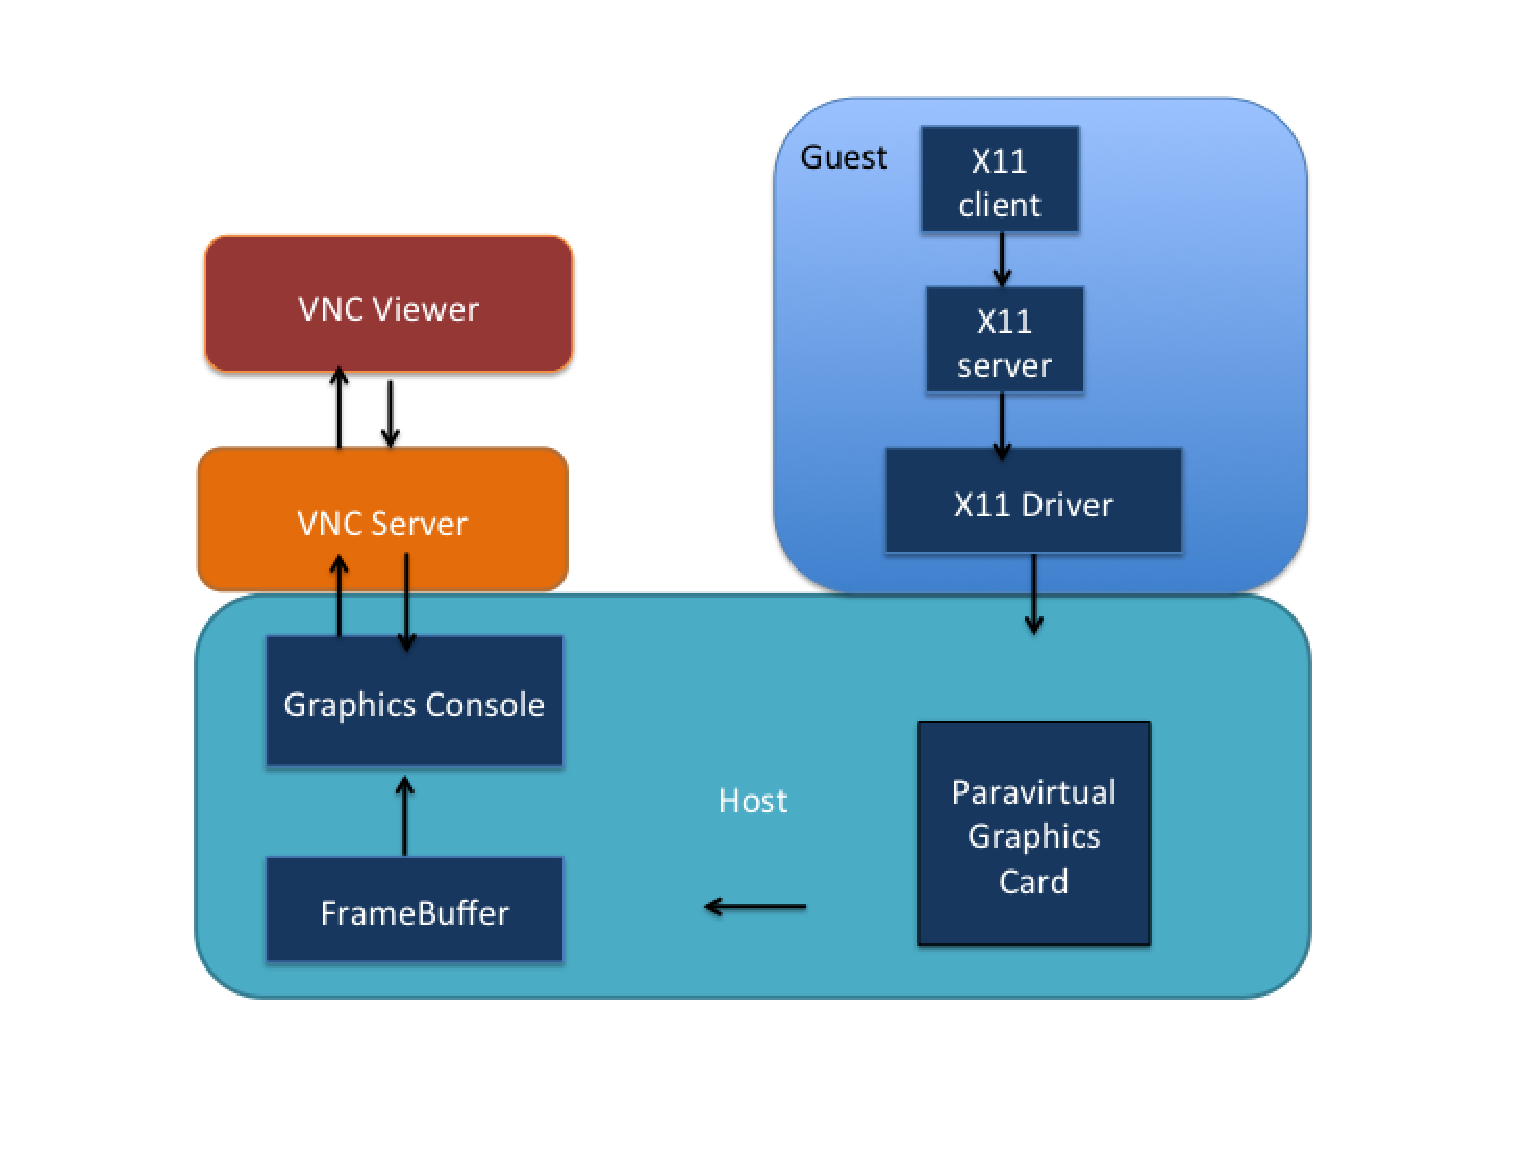
\epsfig{file=Paragraph.eps, height=3in, width=4in}                   
\caption{The new model of graphics in Palacios}   
\end{figure}                                                   
\subsection{ParaGraph: The Paravirtual Graphics Card}
A paravirtual graphics card is essentially a way of representing a graphics card
interface to a virtual guest that is similar but not identical to its hardware
implementation. In our case, we have Paragraph, a virtual graphics card device
that offers the guest a very straightforward interface which is simply: write
the array of pixels. Paragraph's configuration specifies how to write to the
internal array of pixels that Palacios uses to copy from into the frame buffer
that is maintained by the graphics console. \\
\subsubsection{Data Structures}
In order to register Paragraph as a PCI device on the guest, a struct was used
to represent and store Paragraph's state. The struct stores information such as
Paragraph's physical address in the guest, and the size of its mapped region in
pages. It also maintains records regarding the VM, the PCI bus, the VM devices and PCI
devices. If Paragraph is configured to be used as memory, fields for its
physical and virtual addresses are used to store such information. If the
graphics console is used for memory, then the appropriate spec information is
also kept in the paragraph state struct. 
\subsubsection{Configuration}
Paragraph can be set to 1 of 3 modes: \\
\begin{itemize}
\item MEM: Paragraph is used directly as backing memory on which the pixel values
are stored.
\item GCONS\textunderscore MEM: Paragraph is used as backing memory but its contents are
then rendered to the graphic console's frame buffer.
\item GCONSD\textunderscore DIRECT: The graphics console is used directly as memory.
\end{itemize}
When Paragraph is configured to MEM mode, it can be mapped into a chunk of
memory (mmap) and then written to directly. Whatever is written to it will be
passed on to the VNC server and displayed on the screen. When Paragraph is set
to GCONS\textunderscore MEM, whatever gets written on Paragraph will then be
copied to the graphic console's frame buffer (memcpy) and the VNC server will
display its contents on Screen. Finally, if Paragraph is set to GCONS
\textunderscore DIRECT, nothing will be written on the device, the graphic
console will be written to directly.

The Paragraph device projects a graphics console to the guest as a PCI device
Paragraph's length was configured to 4MB and it was given the physical address
of 0x80000000. Paragraph's implementation includes the required initialization
such as registering it as a PCI device, initializing the PCI BAR

Paragraph's implementation is less than 300 lines of code.

\subsection{X11}
 TODO
\subsubsection{X11 Client\--Server Model}

\subsubsection{X11 device driver for Paragraph}
The X11 server requires device drivers to identify and communicate with devices.
In our case, we needed to write a device driver for Paragraph which the X server can
write onto.
X11 drivers come with a set of mandatory functions that they must perform. Table
1 lists these functions.
\section{Results}
The goal of this project was to write a paravirtual graphics card and run an X11
client on the guest that uses this graphics card. Professor Dinda aided us
greatly by providing us with a Paragraph framework that helped us in the first
part, as for running an X11 client, we ran into many issues due to our lack of
experience with X. XWe were able to create a paravirtual graphics card device
that can be configured. 
We were also able to configure an X11 device driver that used such a device as a
frame buffer for the X11 server to render to. However, we still have not been able to run
the X server on the guest, mainly due to our use of a fairly limited guest OS
that don't have all the devices or libraries that the X server needs.
\section{Outstanding Issues}
Running the X server on the virtual guest requires it to be reconfigured. The
use of another guest that has pseudo terminals installed. A
\textit{pseudo\textunderscore terminal} is a special interprocess communication
channel that acts like a terminal. One end of the channel is called the master side or master pseudo-terminal device, 
the other side is called the slave side. 
Data written to the master side is received by the slave side as if it was the result of a user typing at an ordinary terminal, 
and data written to the slave side is sent to the master side as if it was written on an ordinary terminal.
X11 clients such as xterm use pseudo terminals to implement their terminal emulation functionality.

\subsection{Citations}
Citations to articles \cite{bowman:reasoning, clark:pct, braams:babel, herlihy:methodology},
conference
proceedings \cite{clark:pct} or books \cite{salas:calculus, Lamport:LaTeX} listed
in the Bibliography section of your
article will occur throughout the text of your article.
You should use BibTeX to automatically produce this bibliography;
you simply need to insert one of several citation commands with
a key of the item cited in the proper location in
the \texttt{.tex} file \cite{Lamport:LaTeX}.
The key is a short reference you invent to uniquely
identify each work; in this sample document, the key is
the first author's surname and a
word from the title.  This identifying key is included
with each item in the \texttt{.bib} file for your article.

The details of the construction of the \texttt{.bib} file
are beyond the scope of this sample document, but more
information can be found in the \textit{Author's Guide},
and exhaustive details in the \textit{\LaTeX\ User's
Guide}\cite{Lamport:LaTeX}.

This article shows only the plainest form
of the citation command, using \texttt{{\char'134}cite}.
This is what is stipulated in the SIGS style specifications.
No other citation format is endorsed.

\subsection{Tables}
Because tables cannot be split across pages, the best
placement for them is typically the top of the page
nearest their initial cite.  To
ensure this proper ``floating'' placement of tables, use the
environment \textbf{table} to enclose the table's contents and
the table caption.  The contents of the table itself must go
in the \textbf{tabular} environment, to
be aligned properly in rows and columns, with the desired
horizontal and vertical rules.  Again, detailed instructions
on \textbf{tabular} material
is found in the \textit{\LaTeX\ User's Guide}.

Immediately following this sentence is the point at which
Table 1 is included in the input file; compare the
placement of the table here with the table in the printed
dvi output of this document.

\begin{table}
 \centering
  \caption{X11 Driver Functions}
  \begin{tabular}{|l|p{6cm}|} \hline
  Function Name&Description\\ \hline
  ScreenInit & An initialisation function is called from the DIX layer for each screen at the start of each server generation.\\ \hline
  Probe & Identify if there is any hardware present that the driver knows how to drive.\\ \hline
  PreInit & Process information from the xorg.conf file, determine the full characteristics of the hardware, and determine if a valid configuration is present. \\ \hline
  Mode Switch & Change video mode \\ \hline
  ViewPort change & Change the origin of the physical view port \\ \hline
  ScreenSaver state change & Screen saver activation/deactivation \\ \hline
  CloseScreen & A close screen function is called from the DIX layer for each screen at the end of each server generation \\ \hline
\end{tabular}
\end{table}

\begin{table}
\centering
\caption{Frequency of Special Characters}
\begin{tabular}{|c|c|l|} \hline
Non-English or Math&Frequency&Comments\\ \hline
\O & 1 in 1,000& For Swedish names\\ \hline
$\pi$ & 1 in 5& Common in math\\ \hline
\$ & 4 in 5 & Used in business\\ \hline
$\Psi^2_1$ & 1 in 40,000& Unexplained usage\\
\hline\end{tabular}
\end{table}

To set a wider table, which takes up the whole width of
the page's live area, use the environment
\textbf{table*} to enclose the table's contents and
the table caption.  As with a single-column table, this wide
table will ``float" to a location deemed more desirable.
Immediately following this sentence is the point at which
Table 2 is included in the input file; again, it is
instructive to compare the placement of the
table here with the table in the printed dvi
output of this document.


\begin{table*}
\centering
\caption{Some Typical Commands}
\begin{tabular}{|c|c|l|} \hline
Command&A Number&Comments\\ \hline
\texttt{{\char'134}alignauthor} & 100& Author alignment\\ \hline
\texttt{{\char'134}numberofauthors}& 200& Author enumeration\\ \hline
\texttt{{\char'134}table}& 300 & For tables\\ \hline
\texttt{{\char'134}table*}& 400& For wider tables\\ \hline\end{tabular}
\end{table*}
% end the environment with {table*}, NOTE not {table}!

\subsection{Figures}
Like tables, figures cannot be split across pages; the
best placement for them
is typically the top or the bottom of the page nearest
their initial cite.  To ensure this proper ``floating'' placement
of figures, use the environment
\textbf{figure} to enclose the figure and its caption.

This sample document contains examples of \textbf{.eps}
and \textbf{.ps} files to be displayable with \LaTeX.  More
details on each of these is found in the \textit{Author's Guide}.

%\begin{figure}
%\centering
%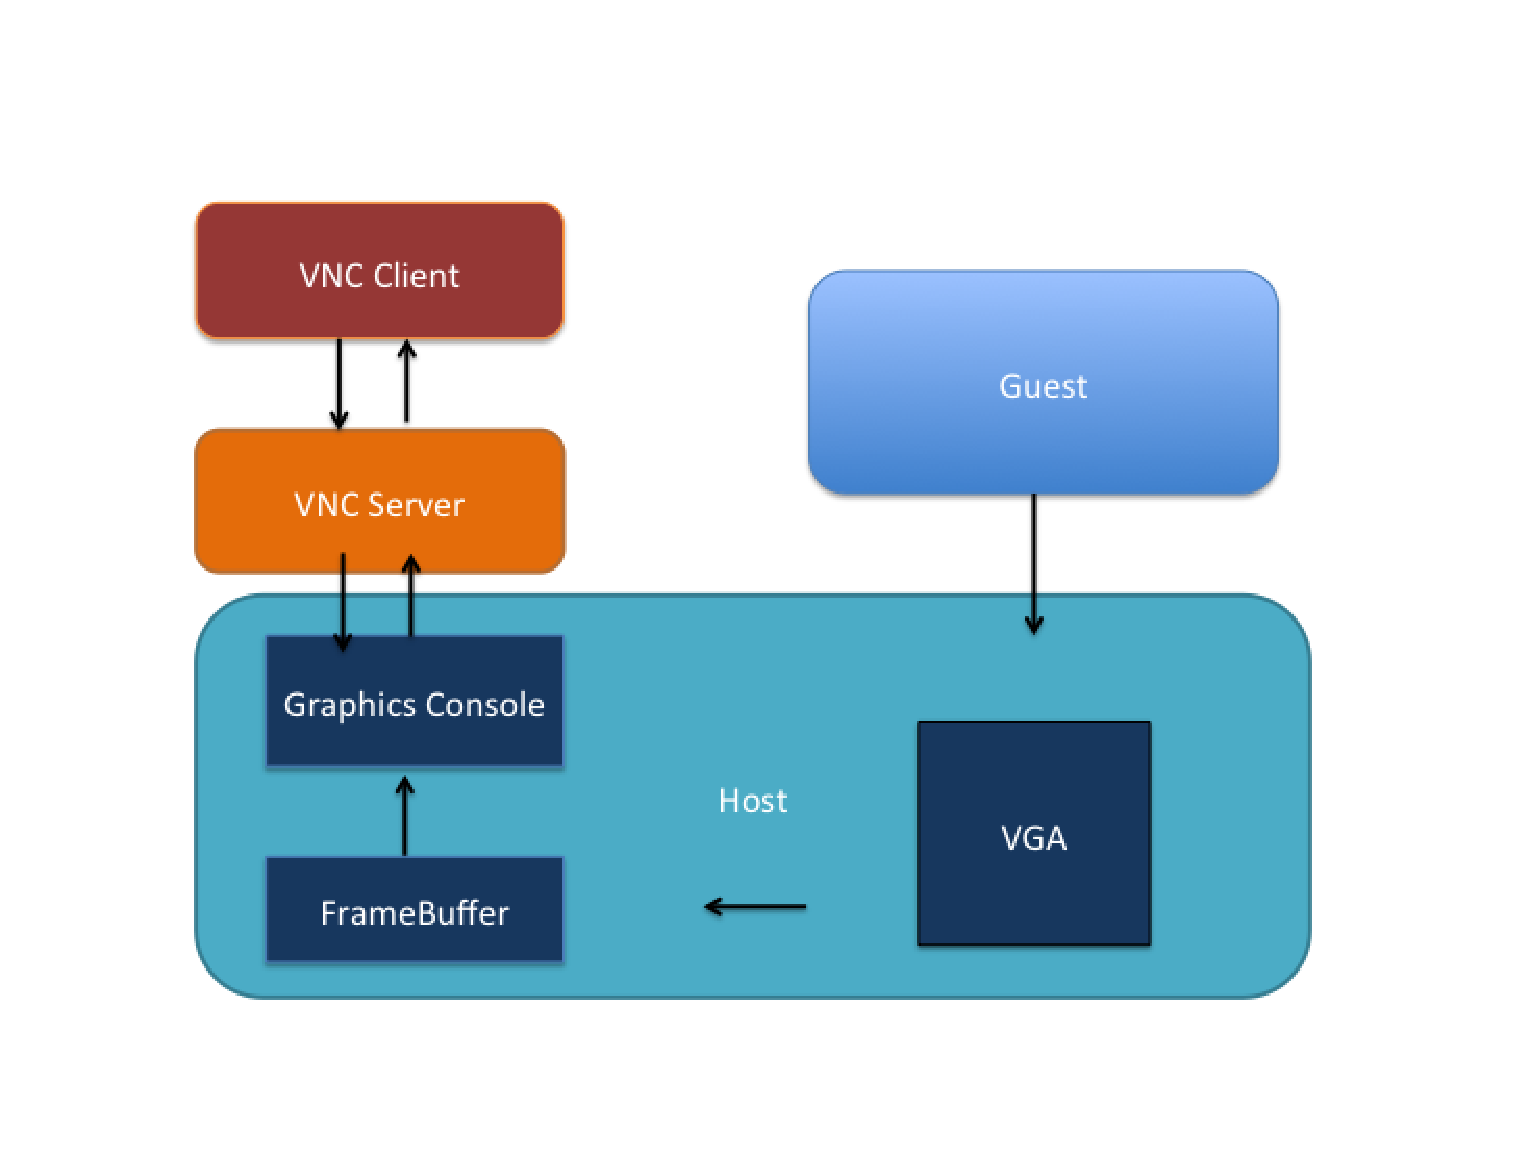
\epsfig{file=VGA.eps}
%\caption{A sample black and white graphic (.eps format).}
%\end{figure}

\begin{figure}
\centering
\epsfig{file=fly.eps, height=1in, width=1in}
\caption{A sample black and white graphic (.eps format)
that has been resized with the \texttt{epsfig} command.}
\end{figure}


As was the case with tables, you may want a figure
that spans two columns.  To do this, and still to
ensure proper ``floating'' placement of tables, use the environment
\textbf{figure*} to enclose the figure and its caption.

Note that either {\textbf{.ps}} or {\textbf{.eps}} formats are
used; use
the \texttt{{\char'134}epsfig} or \texttt{{\char'134}psfig}
commands as appropriate for the different file types.

\section{Conclusions}
This paragraph will end the body of this sample document.
Remember that you might still have Acknowledgments or
Appendices; brief samples of these
follow.  There is still the Bibliography to deal with; and
we will make a disclaimer about that here: with the exception
of the reference to the \LaTeX\ book, the citations in
this paper are to articles which have nothing to
do with the present subject and are used as
examples only.
%\end{document}  % This is where a 'short' article might terminate

%ACKNOWLEDGMENTS are optional
\section{Acknowledgments}
We would like to thank Peter Dinda for the many, many hours he spent tirelessly with us as we
tried to get the X server running on the virtual guest, and for all the
resources and frameworks he provided us with. We would also like to thank Kyle
Hale for sending us all the different guest OS's and reconfiguring them for us
whenever we needed them. Thanks to our diligent undergraduate assistants Prem
Seetharaman, Jack Hudson, and Josiah Matlack for putting up with us during and
not during their office hours.
%
% The following two commands are all you need in the
% initial runs of your .tex file to
% produce the bibliography for the citations in your paper.
\bibliographystyle{abbrv}
\bibliography{sigproc}  % sigproc.bib is the name of the Bibliography in this case
% You must have a proper ".bib" file
%  and remember to run:
% latex bibtex latex latex
% to resolve all references
%
% ACM needs 'a single self-contained file'!
%
%APPENDICES are optional
%\balancecolumns
\appendix
%Appendix A
\section{Headings in Appendices}
The rules about hierarchical headings discussed above for
the body of the article are different in the appendices.
In the \textbf{appendix} environment, the command
\textbf{section} is used to
indicate the start of each Appendix, with alphabetic order
designation (i.e. the first is A, the second B, etc.) and
a title (if you include one).  So, if you need
hierarchical structure
\textit{within} an Appendix, start with \textbf{subsection} as the
highest level. Here is an outline of the body of this
document in Appendix-appropriate form:
\subsection{Introduction}
\subsection{The Body of the Paper}
\subsubsection{Type Changes and  Special Characters}
\subsubsection{Math Equations}
\paragraph{Inline (In-text) Equations}
\paragraph{Display Equations}
\subsubsection{Citations}
\subsubsection{Tables}
\subsubsection{Figures}
\subsubsection{Theorem-like Constructs}
\subsubsection*{A Caveat for the \TeX\ Expert}
\subsection{Conclusions}
\subsection{Acknowledgments}
\subsection{Additional Authors}
This section is inserted by \LaTeX; you do not insert it.
You just add the names and information in the
\texttt{{\char'134}additionalauthors} command at the start
of the document.
\subsection{References}
Generated by bibtex from your ~.bib file.  Run latex,
then bibtex, then latex twice (to resolve references)
to create the ~.bbl file.  Insert that ~.bbl file into
the .tex source file and comment out
the command \texttt{{\char'134}thebibliography}.
% This next section command marks the start of
% Appendix B, and does not continue the present hierarchy
\section{More Help for the Hardy}
The acm\_proc\_article-sp document class file itself is chock-full of succinct
and helpful comments.  If you consider yourself a moderately
experienced to expert user of \LaTeX, you may find reading
it useful but please remember not to change it.
\balancecolumns
% That's all folks!
\end{document}
